\chapter{Background}\label{chap:background}

In this chapter the welding aspects of the problem are explained and previous work is shown regarding the segmentation problem within welding research as well as the use of machine learning algorithms in the field.

Additionally, theoretical background of the deep learning techniques used is shown. For this, an overview of machine learning is given, detailing the problems it tackles and how this approach works in general. Furthermore, different types of Artificial Neural Networks (ANN) are described, namely fully connected networks, convolutional neural networks (CNN) and fully convolutional networks (FCN). 

\section{Welding}

In this thesis the focus is in Gas Metal Arc Welding (GMAW), a welding process in which a consumable electrode is melted by an electric arc. The zone has a shielding gas to prevent external effects in the joint. Figure \ref{fig:gmaw} shows a typical GMAW diagram.

\begin{figure}
    \centering
    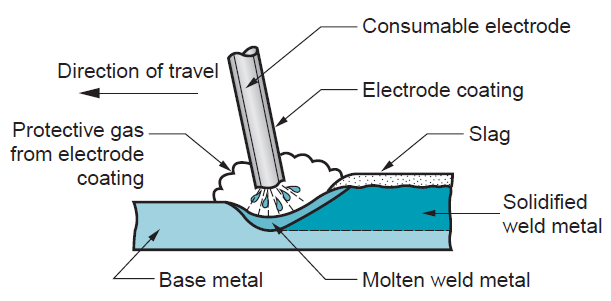
\includegraphics[scale=0.55]{Images/Background/gmaw.png}
    \caption[Illustration of a GMAW process]{GMAW process illustration. Source: \url{https://www.americantorchtip.com/blog/mig-vs-tig}.}
    \label{fig:gmaw}
\end{figure}

The quality of an arc welding operation is highly influenced by the transfer mode. Previous work in GMAW indicates that transfer mode affects weld penetration, weld width, recovery of alloying elements, fume emission, spatter and wetting among others \cite{lancaster, mendez2015}. Furthermore, stable and repeatable transfer modes are achieved by using the correct welding parameters \cite{zhang2}, hence it is important to gain knowledge about the welding dynamics to improve automatic welding systems.

In this thesis, globular and spray transfer modes are considered. Globular transfer consists of large droplets that build up in the end of the consumable electrode untildetachment occurs due to the size. This transfer mode is usually not desirable since it produces high heat, poor welding surfaces and spatter. Nonetheless, it is a cost effective mode because carbon dioxide is used as shielding gas which is cheaper than other gases such as argon. On the other hand, spray transfer uses higher voltage and current, producing a fast melting of the electrode, resulting in small droplets. This increases the quality of the weld and spatter is minimized.

The analysis of welding image data can be useful to understand and design the process. Specifically, it is possible to measure geometric and physical properties which  can provide useful information when designing and optimizing a GMAW process as well as characterizing it. Furthermore, this can help to study mathematical descriptions of droplet flight and better development of automatic welding systems.

\subsection{Previous work}

The use of high speed video welding data has been explored before, using computer vision techniques that can detect the contour of objects within an image, with the aim of obtaining characteristic features of the metal droplets. 

In \textit{Ray et al.} \cite{Ray} an active contour model, also known as \textit{snakes}, was used and was able to accurately outline the border of a droplet. This is a method for outlining an image object and it is widely used in object tracking, shape recognition and edge detection. It is an analytic method in which a set of seeded splines are moved in the image by minimizing an energy function which depends on features of the image, namely lines, edges and terminations; the energy minimum is reached when the points of the spline are able to outline the shapes in the image \cite{Kass} as shown in figure \ref{fig:snakes}.

\begin{figure}
\centering
  \begin{subfigure}[b]{0.45\textwidth}
    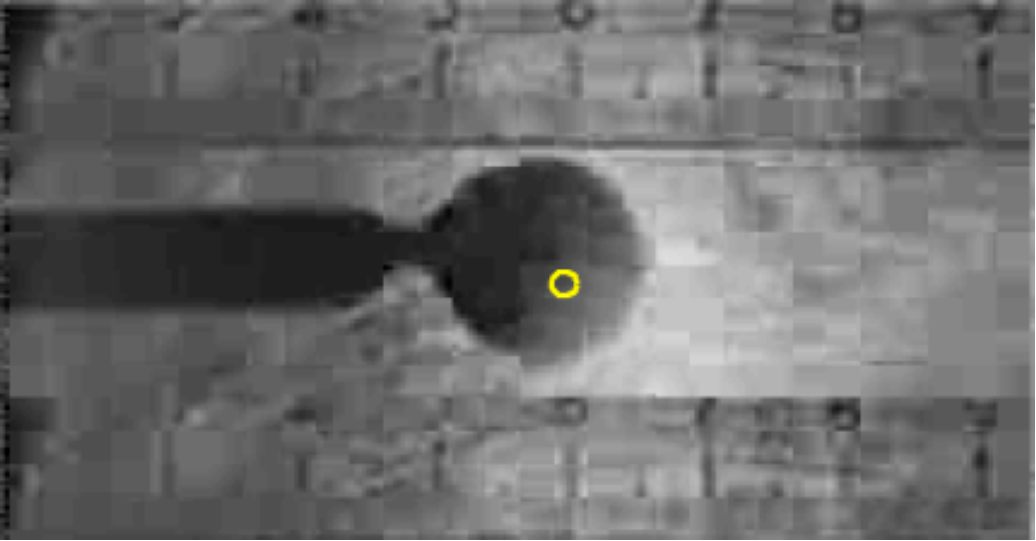
\includegraphics[width=\linewidth]{Images/Background/snake_a.png}
    \caption{Snake seed}
    \label{fig:snake_a}
  \end{subfigure}
\hfill
  \begin{subfigure}[b]{0.45\textwidth}
    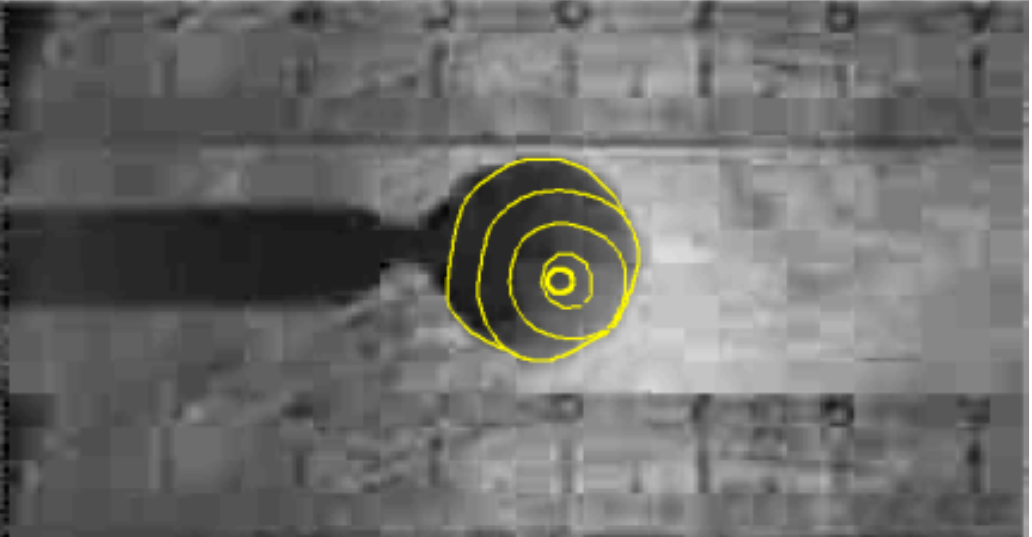
\includegraphics[width=\linewidth]{Images/Background/snake_b.png}
    \caption{Evolution of snake from the seed}
    \label{fig:snake_b}
  \end{subfigure}
  \begin{subfigure}[b]{0.45\textwidth}
    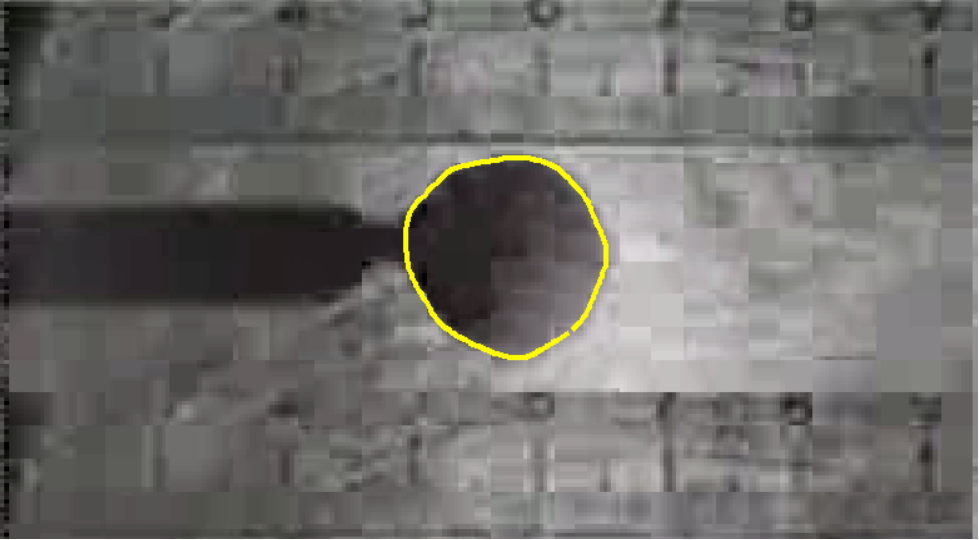
\includegraphics[width=\linewidth]{Images/Background/snake_c.png}
    \caption{Final evolved snake}
    \label{fig:snake_c}
  \end{subfigure}
  \caption[Snake methodology application]{Snake methodology used in \textit{Ray et al.} \cite{Ray}}
  \label{fig:snakes}
\end{figure}

Another case of GMAW droplet segmentation is in \textit{Zhai} \cite{Zhai} in which the problem is solved by using standard techniques of computer vision. Several image enhancement filters were applied to the image in a pipeline, such as grayscaling, thresholding, edge operators (Sobel operator, Laplacian of Gaussian operator, Canny operator among others) and histogram equalization in order to separate the droplet from the background. This approach has a different process for attached and detached droplets. 

Furthermore, in the work of \textit{Wang} \cite{wang}, a similar approach to \textit{Zhai} \cite{Zhai} was used, that is applying successive filters to the images to get a proper segmentation. Then, location and size of the droplet were measured accurately.

While the droplets were properly segmented in the examples mentioned above, this was done in a per image fashion, this means that to analyze thousands of images one would have to run the model thousands of times which is time consuming\footnote{In the work of \textit{Wang} \cite{wang} it is stated that the speed could be greatly improved by migrating from Matlab based code to C, but this is not done in the paper.}. Also, in \textit{Zhai} \cite{Zhai}, different models are needed for attached and detached droplets. Therefore it is necessary not only to properly segment, but to be able to process a large amount of images in a more general approach.

Although deep learning techniques have been used in welding imaging problems, it has been mainly in a reinforcement learning approach to control the welding machine \textit{in situ} \cite{Gunther}. Similarly, neural networks have been used for defect detection using several sensors, this was achieved with the use of Convolutional Neural Networks to classify the input into one of different degrees of quality of the result, that is to say modes of failure \cite{Zhang}. Recently, deep learning has also been used for weld bead geometry prediction \cite{bead}.

Nonetheless, to the best of the author's knowledge, segmentation problems have not been addressed with the use of deep learning techniques in the study of welding video data, which makes this thesis a novel approach to help solving a relevant problem in the field.

\section{Machine Learning}

Machine Learning is a field within Artificial Intelligence which aims to solve tasks automatically by learning patterns from data as opposed to hard-coding specific instructions or employing analytical models. In an abstract way, the learning characteristic can be defined as follows \cite{Mitchell}: “A computer program is said to learn from experience E with respect to some class of tasks T and performance measure P, if its performance at tasks in T, as measured by P, improves with experience E”.

 The task (T) is what the computer has to do, and it gets better at it by processing examples of said task, in other words, gaining experience (E) in the task. The examples are the input of the model, and usually come in the form of a vector $x \in \R^n$. For example, if the input data are RGB images, then $x \in R^3$ and has dimensions $(width,\hspace{2pt} height, \hspace{2pt} channels)$ and each data point in $x$ is a pixel value. Another example is when each column of $x$ represents a specific feature relevant to the task.

Typical machine learning tasks are the following:
\begin{itemize}
    \item \textbf{Classification:} The task is to assign the input to a specific set of outputs by tuning the parameters of a function such that: $f: \R^n \xrightarrow{} \{1,\ldots, k\}$ where $k$ is the number of possible classes. An example of this is the handwritten digits problem \cite{MNIST}, in which an image of a handwritten digit is given and the output is which class ($\{0,\ldots,9\}$) the model is assigning to it. 
    \item \textbf{Regression:} In this case, the model's task is to learn a function $f: \R^n\xrightarrow{}\R$. The output is not a finite set of values, but a continuous value. Examples of this are when the task is to predict some physical measurement in the future with historical data like predicting tomorrow's temperature (continuous output) based on recent climate data trends.
    \item \textbf{Anomaly detection:} This case is similar to classification, since the task is to flag abnormal data from the rest.The difference lies in the fact that there is one class that is larger than the rest and sometimes the large class is the only class present in the training phase. This can be used to prevent fraudulent use of credit cards (abnormal data). 
    \item \textbf{Denoising}: For this case the model learns to represent normal or baseline data, so that when a corrupted example is given, the model can reduce the noise in the corrupted example.
\end{itemize}

The performance measure (P) is important since it is the metric that the model will use to effectively learn from the given examples. In classification tasks, P can be the accuracy, that is how many correct predictions were made out of the total examples. In the case of regression it makes more sense to use a distance metric to measure how far away the predicted value is from the real value. In anomaly detection, since one class is way larger than the other, accuracy can be deceiving and other metrics are used such as the F1-score. However, choosing an appropriate metric is not always straightforward and it is important to understand the task and the nature of the data to decide which metric would be more effective \cite{loss-survey}.

Another important aspect is that the performance measure that matters is the one computed in new data, since training data has already been seen, it is expected that the error is going to be small when measured using that data, or at least smaller than in the unseen data. Because of that, datasets are usually split into training and testing sets.

Finally, the experience (E) will also determine how to approach the problem. The type of data (experience) can be categorized as follows:
\begin{itemize}
    \item \textbf{Supervised learning:} The data consists of pairs $(x,y)$ in which $x$ is the input and $y$ is the correct output for $x$. In the handwritten digits examples, a data point would be $x$, an image with a hand drawn digit $n\in \{0,\ldots,9\}$, and $y$, the integer number $n$.
    \item \textbf{Unsupervised learning:} In this case, no ground truth data is given, only the input $x$. This can be useful to explore the structure of the data itself by learning representations of it. Also it is used when one does not know how to categorize the data and lets the model cluster similar examples which can be useful, for example, when categorizing customer preferences or categorizing texts.
    \item \textbf{Reinforcement learning:} In this case the data is constantly being fed to an agent that makes decisions based on the stream of data. This is used for optimal control purposes, in which the agent must react to different scenarios by changing its behavior such as in self-driving cars.
\end{itemize}

It is important to note that supervised learning is more “expensive” compared to unsupervised, since labels are not always available, and it is often the case that manual labels need to be made in order to train in a supervised approach, which can be slow when the data is large. Nonetheless, supervised learning allows to have more accurate results, since the exact\footnote{This will depend on the task at hand. Especially when manually labeling data, the ground truth can have bias of the scientist that is labeling. For example in image segmentation, in which the boundaries between subjects are not a clear pixel-wise separation.} result is given to the model, hence it is possible for the network to reach a high performance.

\section{Artificial Neural Networks}

An Artificial Neural Network (ANN) is a mathematical model that learns a function $y = f(x;w)$ where $y$ is an output (prediction), $x$ is an input and $w$ are the parameters (or weights) of $f$. The network learns parameters $w$ such that $f\approx f^*$ where $f^*$ is the function that correctly maps input to output.

These kinds of models are said to be layered since the function $f(x; w)$ is usually a composition of several non-linear transformations and each composition is thought of as a layer of the model. Then $f$ can be represented as 
\begin{align}
    f(x;w) = f^{(n)}(f^{(n-1)}(\ldots f^{(2)} (f^{(1)}(x;w)))
    \label{eq:layers}
\end{align}
Thus, the data flows in a feedforward fashion from the first layer or input layer $f^{(1)}$ through the \textit{hidden layers} of the network until the last layer $f^{(n)}$ which is the output layer. The use of deeper composition chains is known as \textit{deep learning}.

In a supervised context, the model looks for a function $f(x) \approx f^*(x)$ where the training data is a noisy approximation of $f^*(x)$. The data consists in pairs $(x, y)$ where $y \approx f^*(x)$, so the input and output layers are determined, and the model tunes the parameters in the hidden layers in order to get an accurate output.

The “neural” characteristic comes from a loose analogy to how biological neurons work, in which a sensory input is given, then a feedforward chain of neurons fire to propagate the information to the brain so that it can perceive and make sense of the input. Also, neurons have a trigger, namely an action potential which works by differences in voltage in order to be activated. In ANN these triggers are the activation functions which originally resembled this action potential behavior by using logistic functions in which extreme values tend to “collapse” to specific values, emulating the not triggered/triggered states.

\begin{figure}
  \begin{subfigure}[b]{0.4\textwidth}
    \def\layersep{3cm}

\begin{tikzpicture}[shorten >=1pt,->,draw=black!50, node distance=\layersep]
    \tikzstyle{every pin edge}=[<-,shorten <=1pt]
    \tikzstyle{neuron}=[circle,draw=black,minimum size=20pt,inner sep=0pt, line width=.4pt]
    \tikzstyle{input neuron}=[neuron, fill=green!20];
    \tikzstyle{bias neuron}=[neuron, fill=gray!20];
    \tikzstyle{output neuron}=[neuron, fill=red!20];
    \tikzstyle{hidden neuron}=[neuron, fill=blue!20];
    \tikzstyle{annot} = [text width=4em, text centered]

    % Draw the input layer nodes
    \foreach[count=\i from 0] \name / \y in {4,3, 0}
    % This is the same as writing \foreach \name / \y in {1/1,2/2,3/3,4/4}
        \ifthenelse{\i=0}{  \node[bias neuron, pin=left:$x_\i$] (I-\name) at (0,-\y-.5) {}}{ \ifthenelse{\i=2}{  \node[input neuron, pin=left:$x_D$] (I-\name) at (0,-\y-.5) {}}{  \node[input neuron, pin=left:$x_\i$] (I-\name) at (0,-\y-.5) {}}}
          ;

    % Draw the hidden layer nodes
    \foreach[count=\i from 0] \name / \y in {5,4,1}
        \ifthenelse{\i=0}{ \path[yshift=0.5cm]
            node[bias neuron] (H-\name) at (\layersep,-\y cm) {}}{\ifthenelse{\i=2}{ \path[yshift=0.5cm]
            node[hidden neuron] (H-\name) at (\layersep,-\y cm) {}}{ \path[yshift=0.5cm]
            node[hidden neuron] (H-\name) at (\layersep,-\y cm) {}}}
       ;
    
    % Draw the output layer nodes
    \foreach[count=\i from 1] \name / \y in {4,1}
        \ifthenelse{\i=2}{\path[yshift=0.5cm]
        node[output neuron] (O-\name) at (2*\layersep,-\y cm) {}}{\path[yshift=0.5cm]
        node[output neuron] (O-\name) at (2*\layersep,-\y cm) {}};
        
    % Connect every node in the input layer with every node in the
    % hidden layer.
    \foreach[count=\i from 0] \source in {4,3,0}
        \foreach[count=\j from 0] \dest in {5,4,1}
        \ifthenelse{\i=0 \AND \j=0 \OR \j=0}{}{\path (I-\source) edge (H-\dest)};

        % Connect every node in the hidden layer with the output layer
    \foreach \source in {5,4,1}
        \foreach \dest in {4,1}
        \path (H-\source) edge (O-\dest);
    % Annotate the layers
    \node[annot] at (\layersep, 1) {Hidden layer};
    \node[annot] at (0,1) {Input layer};
    \node[annot] at (2*\layersep, 1) {Output layer};
    
    \node[annot] at (0.8*\layersep,-0.1) {$z_M$};
    \node[annot] at (0.8*\layersep,-3.2) {$z_1$};
    \node[annot] at (0.8*\layersep,-4.6) {$z_0$};
    
    \node[annot] at (2.2*\layersep,-0.1) {$y_K$};
    \node[annot] at (2.2*\layersep,-3.2) {$y_1$};
    
    \node[annot] at (0.5*\layersep,0) {$w^{(1)}_{MD}$};
    \node[annot] at (1.5*\layersep,0) {$w^{(2)}_{KM}$};
    \node[annot] at (1.5*\layersep,-4.3) {$w^{(2)}_{10}$};
    
    
    \foreach \i in {-1,-1.4,-1.8,-2.2,-2.6,-3}
        \node[circle,draw=black,minimum size=2pt,inner sep=0pt, fill=black!50] at (0,\i) {};
    \foreach \i in {-1,-1.4,-1.8,-2.2,-2.6,-3}
        \node[circle,draw=black,minimum size=2pt,inner sep=0pt, fill=black!50] at (\layersep,\i) {};
    \foreach \i in {-1,-1.4,-1.8,-2.2,-2.6,-3}
        \node[circle,draw=black,minimum size=2pt,inner sep=0pt, fill=black!50] at (2*\layersep,\i) {};
\end{tikzpicture}

    \caption{Two layer neural network diagram}
    \label{fig:ann}
  \end{subfigure}
\hfill
  \begin{subfigure}[b]{0.4\textwidth}
    \def\layersep{3cm}
\def\maxheight{2.1}
\def\dotoffset{1.55}
\def\hoffset{0}
\newcommand*{\Scale}[2][4]{\scalebox{#1}{$#2$}}%
\begin{tikzpicture}[shorten >=1pt,->,draw=black!50, node distance=\layersep]
    \tikzstyle{every pin edge}=[<-,shorten <=1pt]
    \tikzstyle{neuron}=[circle,draw=black,minimum size=20pt,inner sep=0pt, line width=.4pt]
    \tikzstyle{input neuron}=[neuron, fill=blue!20];
    \tikzstyle{bias neuron}=[neuron, fill=gray!20];
    \tikzstyle{output neuron}=[neuron, fill=red!20];
    \tikzstyle{hidden neuron}=[circle split,draw=black,minimum size=40pt,inner sep=0pt, line width=.4pt]
    \tikzstyle{annot} = [text width=4em, text centered]

    % Draw the input layer nodes
    \foreach[count=\i from 0] \name / \y in {4,3, 0}
    % This is the same as writing \foreach \name / \y in {1/1,2/2,3/3,4/4}
        \ifthenelse{\i=0}{  \node[bias neuron] (I-\name) at (\hoffset,-\y+\maxheight) {$z^{(l)}_\i$}}{ \ifthenelse{\i=2}{  \node[input neuron] (I-\name) at (\hoffset,-\y+\maxheight) {$z^{(l)}_M$}}{  \node[input neuron] (I-\name) at (\hoffset,-\y+\maxheight) {$z^{(l)}_\i$}}}
          ;
    
    \node[annot] at (1+\hoffset, 2) {$w^{(l)}_{nM}$};
    \node[annot] at (\hoffset+.6, -.2) {$w^{(l)}_{n1}$};
    \node[annot] at (1+\hoffset, -1.8) {$w^{(l)}_{n0}$};
        
    \node[hidden neuron, rotate=90] (H-i) at (1+\hoffset+\layersep, -2+\maxheight) {\rotatebox{-90}{$\overset{M}{\underset{j=1}{\sum}}w_{nj}z^{(l)}_j$}
     \nodepart{lower} \rotatebox{-90}{$\quad h(a_n)$}};
     
     \path (H-i) edge (2.2*\layersep+1+\hoffset,-2+\maxheight);
    

        
    % Connect every node in the input layer with every node in the
    % hidden layer.
    \foreach \source in {4,3,0}
        \path (I-\source) edge (H-i);

    % Annotate the layers
    \node[annot] at (1+\hoffset+\layersep, 3.3) {Layer $l+1$, Neuron $n$};
    \node[annot] at (\hoffset,3.7) {Layer $l$};
    \node[annot] at (1+ 1+\hoffset+ 1.8*\layersep, -1.5+\maxheight) {$z_n^{(l+1)}$};

  \foreach \i in {-.1,-0.55, -1, -1.45, -1.9}
    \node[circle,draw=black,minimum size=2pt,inner sep=0pt, fill=black!50] at (\hoffset,\i+\dotoffset) {};
        
\end{tikzpicture}

    \caption{Neuron unit}
    \label{fig:feed_forward}
  \end{subfigure}
  \caption[Illustration of a two layer fully connected neural network (a) and a neuron unit (b)]{A two layer neural network diagram is shown in (a). Nodes represent input (green), hidden (blue) and output (red) variables while links represent the weights between nodes in which a bias (gray) weight is added. In (b), the feed forward calculation is shown from a given layer $l$ to a neuron in the following layer. First computing the linear combination of inputs and then applying an activation function. }
\end{figure}

In figure \ref{fig:ann} is a simple ANN of two layers\footnote{The way of counting layers can be somewhat arbitrary, since one could include everything and consider a three layer network, or only include hidden layers, in which case the network has one layer. The convention here is to count the number of layer connections, since this reflects the parameters that the network will optimize. Hence, it is considered a two layer network.} is shown. This kind of network is called a dense or fully connected network, since every node in one layer is connected to every node in the next layer. In a given layer, each neuron will output an activation value to each of the neurons in the next layer through a linear combination of the inputs $x_i$ and the respective weights $w^l_{ji}$. Once the activations are calculated, these are fed to a non-linear activation function producing the new values to be received by the next layer\footnote{In figure \ref{fig:feed_forward}, $h(\cdot)$ is shown as single function, but in principle there could be many different functions. The indices $h^{(l)}_n(\cdot)$ that indicate layer (l) and neuron (n) are omitted for simplicity.}. Then, in the first layer with $D$ neurons, the activations of the second layer are given by
\begin{align*}
    a_j = \sum^D_{i=1}w^{(1)}_{ji}x_i+w^{(1)}_{j0}, \quad j \in \{1,\ldots, M\}
\end{align*}
where $M$ is the number of neurons in the second layer and $D$ is the number of neurons in the input layer. Also, the superscript $(1)$ indicates that the parameters are from the first layer. The parameters $w_{ji}$ are the weights connecting the neuron $j$ from the second layer and the neuron $i$ from the first layer. The parameters $w_{j0}$ are biases which serve as an offset to the activation. Later, the activations are transformed using an activation function
\begin{align*}
    z_j = h(a_j)
\end{align*}
where $h(\cdot)$ is a nonlinear function such as the sigmoid or hyperbolic tangent.

Conversely, the output layer can be computed from the previous layer as
\begin{align*}
    a_k = \sum^M_{j=1}w^{(2)}_{kj}z_j+w^{(2)}_{k0}, \quad k \in \{1,\ldots, K\}
\end{align*}
where $K$ is the number of outputs and $z_j$ are the results of the previous layer. Finally, the output activations must be transformed to map the type of the output data. In a regression problem no transformation is needed, so the identity function is used and $y_k = a_k$. In the case of classification it is necessary to use a function to cast the activations into specific classes
\begin{align*}
    y_k &= \sigma (a_k)\\
    \sigma(a_k) &= \frac{e^{a_i}}{\sum^K_{j=1}e^{a_j}}
\end{align*}
where $\sigma(\cdot)$ is the \textit{softmax} function, a generalization of the sigmoid for the multiple class case, and it measures the probability $p(C_i|x)$, the probability that the output belongs to class $C_i$,  where $i=1,\ldots, K$, given the input $x$.

Then, the final output of the network can be expressed as 
\begin{align}
    y_k(\mathbf{x},\mathbf{W}) = \underbrace{\sigma_k \left(\sum^M_{j=1}w^{(2)}_{kj}\underbrace{h\left(\sum^D_{i=1}w^{(1)}_{ji}x_i+w^{(1)}_{j0}\right)}_{f^{(1)}(x)}+w^{(2)}_{k0}\right)}_{f^{(2)}(f^{(1)}(x))}, \quad k \in \{1,\ldots, K\}
    \label{eq:neural_net}
\end{align}
and by using matrix notation we get the more compact version
\begin{align*}
    \mathbf{z}^{(1)} &= h^{(1)}\left(\mathbf{W}^{(1)T}\mathbf{x} + \mathbf{b}^{(1)}\right) \\
    \mathbf{y}(\mathbf{x},\mathbf{W})&= \sigma\left(\mathbf{W}^{(2)T}\mathbf{z}^{(1)} + \mathbf{b}^{(2)}\right)
\end{align*}
In equation \eqref{eq:neural_net} it can be seen more explicitly the relationship with the abstract form of expression \eqref{eq:layers} in which the composition of functions represents the layered structure. Furthermore, deeper architectures can be made simply by adding further compositions of the functions representing each layer. In general, a fully connected neural network of $L$ layers can be expressed as
\begin{align*}
    \mathbf{z}^{(1)} &= h^{(1)}\left(\mathbf{W}^{(1)T}\mathbf{x} + \mathbf{b}^{(1)}\right) \\
    \mathbf{z}^{(l)} &= h^{(l)}\left(\mathbf{W}^{(l)T}\mathbf{z}^{(l-1)} + \mathbf{b}^{(l)}\right), \quad l \in \{2,\ldots, L-1 \} \\
    \mathbf{y}(\mathbf{x}, \mathbf{W})  &=\sigma\left(\mathbf{W}^{(L)T}\mathbf{z}^{(L-1)} + \mathbf{b}^{(L)}\right) 
\end{align*}
where each equation represents input layer, hidden layers and output layer respectively.

\subsection{Activation functions}

An important aspect of the neural network's architecture is that it needs to have a non-linear transformation to be able to approximate functions that can be extremely complex \cite{Hornik, Cybenko}. The most commonly used activation functions are the rectified linear unit (ReLU), leaky ReLU, sigmoid and hyperbolic tangent. These functions are shown in figure \ref{fig:activations}. In practice, the most used are the ReLU and leaky ReLU because the derivative of the sigmoid and hyperbolic tangent tends to zero on the edges, which means that the deeper the network, the closer the gradients are to zero and then it is not possible to update the weights since gradient computation is a fundamental step to optimize the weights. This is known as the vanishing gradients problem and is especially present when using deep learning models \cite{vanishing-gradient, Hinton2010}.

These functions are defined as
\begin{align*}
    sigmoid(x)=\sigma(x) &= \frac{1}{1+e^{-x}} \\
    tanh(x) &= \frac{e^x-e^{-x}}{e^x+e^{-x}} \\
    ReLU(x) &= max(0,x)\\
    LeakyReLU(x) &= max(\alpha x, x),\quad 0<\alpha < 1
\end{align*}
\begin{figure}
    \centering
    \begin{tikzpicture}[domain=-2.9:2.9]
        % grid
        \draw[very thin,color=gray] (-2.9, -1.1) grid (2.9, 2.9);
        \foreach \x in {-2,-1,0,1,2}
            \node[anchor=north] at (\x,-1.1) {\x};
        \foreach \y in {-1,0,1,2}
            \node[anchor=east] at (-2.9,\y) {\y};
        % axes
        \draw[->,thick] (-2.9, 0) -- (3.1, 0) node[right] {$x$};
        \draw[->,thick] (0, -1.1) -- (0, 3.1) node[above] {$f(x)$};

        % Logistic
        \draw[thick, color=blue]
            plot (\x, { 1/(1+exp(-1 * \x)) })
            node[right,yshift=-0.5em] {$\sigma(x)$};
        % Beta logistic
        %\draw[color=purple] plot (\x, { 1/(1+exp(-.5 * \x)) })
        %    node[right] {$logistic(a), beta=.5$};
        % Tanh
        \draw[thick, color=orange]
            plot (\x, { ( 1 - exp(-2*\x) ) / ( 1 + exp(-2*\x) ) })
            node[right,yshift=0.5em] {$tanh(x)$};
        
        % Leaky ReLU
        \draw[thick, color=black!70]
            plot (\x, { max(0.08 * \x, \x) })
            node[xshift=-19.3em,yshift=-8em] (a) {$Leaky ReLU(x)$};
            
        % ReLU
        \draw[thick, color=red]
            plot (\x, { max(0, \x) })
            %node[right] {$ReLU(x)$};
            node[below = -1.2em of a.east, anchor=east] {$ReLU(x)$};
            
    \end{tikzpicture}
    \caption[Commonly used activation functions]{Commonly used activation functions. Sigmoid, hyperbolic tangent, ReLU and Leaky ReLU. ReLU and Leaky ReLU overlap when $x\geq0$.}
   \label{fig:activations}
\end{figure}

\subsection{Training}
In the previous sections the way in which the network computes an output from a given input has been shown. However, for the network to be useful it is necessary to tune the weights so that the model can accurately make predictions. This process of tweaking parameters is called the training phase. A dataset is usually split into at least two groups: training set and testing set. So that the model can optimize parameters by receiving the training data and then using the testing data to measure some performance metric, thus measuring how good the model is at generalization.

In the training phase, it is necessary to optimize the weights such that some error function\footnote{Also called loss or cost function.} is the smallest possible. That is solving the problem 
\begin{align*}
    \mathbf{W}^*=\underset{\mathbf{W}}{arg\,min}\:E(\mathbf{W};\mathbf{X})
\end{align*}
Although it is possible in theory to solve the minimization problem by calculating the gradient of $E(\cdot)$ analytically and then solving for $\nabla E(\mathbf{W};\mathbf{X})=0$, it is often too computationally expensive, and iterative methods are preferred. 

In order to achieve this iterative minimization, the \textit{backpropagation} algorithm is used which efficiently computes the gradient of an error function with respect to the weights of the network for an input-output example. Since the error is calculated in the last layer, after the feedforward pass, the gradient is calculated backwards, from the output layer to the input layer, propagating the error using the chain rule at each layer. A more detailed discussion of the backpropagation algorithm can be found in \textit{Goodfellow} and \textit{Bishop} \cite{dl-book, bishop}.

After backpropagation, it is possible to use optimization methods to find weights that minimize the error $E(\cdot)$. One way to solve this problem is to use gradient descent methods. Specifically, the Stochastic Gradient Descent (SGD) method is a common approach. In SGD, weights are initialized randomly, then each iteration tunes the weights such that the value of the error is updated in the opposite direction of the gradient, thus reducing its value.

If the weight matrix is $\mathbf{W} \in \R^P$, then the partial derivatives of $E(\cdot)$ are
\begin{align*}
    \frac{\partial E}{\partial \mathbf{W}}=\left[\frac{\partial E}{\partial w_1}, \ldots, \frac{\partial E}{\partial w_P}\right]^T
\end{align*}
subsequently, the weights are updated as follows
\begin{align}
    w_i \xrightarrow{} w_i - \alpha \frac{\partial E}{\partial w_i},\quad \forall i \in \{1,\ldots, P\} 
    \label{eq:sgd}
\end{align}
where $\alpha$ is the learning rate, which determines how large the steps are between iterations. A smaller value will produce a slower but more accurate algorithm. Conversely, a larger learning rate will increase speed, but minima are harder to find. The weights are updated until the error is close to zero by using some tolerance measure.

Equation \eqref{eq:sgd} implies that a single pair $(x,y)$ is processed by the network, this is often not optimal because datasets can have a large number of data points, so a variant of SGD is used called mini-batch gradient descent in which the data is split into many small bacthes and the gradient descent is done over the average of the gradients within the batch. Finally, the updating rule for a batch is
\begin{align*}
    w_i \xrightarrow{} w_i - \frac{\alpha}{N} \sum_{j=0}^N\frac{\partial E_j}{\partial w_i},\quad \forall i \in \{1,\ldots, P\} 
\end{align*}
where the sum is done over all the examples in the batch. Furthermore, there are many optimizers aside from SGD which incorporate more levels of sophistication such as using momentum or decaying learning rate. Some of them are AdaGrad, Adadelta and Adam, the latter being particularly common.

Then, to optimize the network this process needs to be repeated for a number of epochs that yields good results. An epoch is defined as the number of times the model has processed the training data, since it is usually necessary to process the training data many times before achieving acceptable results.

\subsection{Regularization}

An important trade-off when training neural network is underfitting-overfitting. Briefly, these concepts convey the idea of how much does the network learn specifically the training data as opposed to generalizing to unseen data. Underfitting means that the network lacks the ability to perform well in the task, but has similar results both in training data as well as testing data. On the other hand, overfitting occurs when the model is too complex and it is able to have really good results in training data but at the cost of not being able to generalize, thus yielding bad results when testing. In figure \ref{fig:overfit} an illustration of the underfitting-overfitting phenomena is shown.

In general, overfitting is more common in deep learning because the models are usually large and contain millions of parameters. The techniques used to address these problems are referred to as regularization techniques.

\begin{figure}
    \centering
    \resizebox{\linewidth}{!}{
    \begin{tikzpicture}[font=\sffamily,
declare function={f(\x)=0.5*pow(abs(\x-2),2)-0.06*pow(\x-2,3);}]
 \foreach \Z in {1,...,42}
 {\pgfmathsetmacro{\X}{\Z/10}
 \pgfmathsetmacro{\Y}{f(\X)+0.9*rnd}
 \ifnum\Z=1
  \xdef\LstOne{(\X,\Y)}
  \xdef\LstTwo{"(\X,\Y)"}
 \else
  \xdef\LstOne{\LstOne (\X,\Y)}
  \xdef\LstTwo{\LstTwo,"(\X,\Y)"}
 \fi}
%  \begin{scope}[local bounding box=over0]
%  \foreach \Z in {1,...,42}
%  {\pgfmathsetmacro{\Coor}{{\LstTwo}[\Z-1]}
%  \fill \Coor circle[radius=1pt];
%  }
%  \draw plot[smooth] coordinates \LstOne;
%  \end{scope}
 \begin{scope}[local bounding box=over,xshift=-5cm]
 \foreach \Z in {1,...,40}
 {\pgfmathsetmacro{\Last}{{\LstTwo}[\Z-1]}
 \pgfmathsetmacro{\Current}{{\LstTwo}[\Z]}
 \pgfmathsetmacro{\Next}{{\LstTwo}[\Z+1]}
 %\typeout{\Last,\Current,\Next}
  \edef\temp{\noexpand\path ($0.6*\Current+0.2*\Last+0.2*\Next$)   coordinate 
  (p\Z);}
  \temp
  \ifnum\Z=1
  \xdef\LstThree{(p\Z)}
  \else
  \xdef\LstThree{\LstThree (p\Z)}
  \fi
  }
 \foreach \Z in {1,...,42}
 {\pgfmathsetmacro{\Coor}{{\LstTwo}[\Z-1]}
 \fill \Coor circle[radius=1pt];
 }
 \draw[thick,blue] plot[smooth] coordinates \LstThree;
 \end{scope}
 %
 \begin{scope}[local bounding box=good,xshift=-10cm]
 \foreach \Z in {1,...,42}
 {\pgfmathsetmacro{\Coor}{{\LstTwo}[\Z-1]}
 \fill \Coor circle[radius=1pt];
 }
 \draw[thick,blue] plot[smooth,domain=0.1:4.2,variable=\x] (\x,{f(\x)+0.45});
 \end{scope}
 %
 \begin{scope}[local bounding box=under,xshift=-15cm]
 \foreach \Z in {1,...,42}
 {\pgfmathsetmacro{\Coor}{{\LstTwo}[\Z-1]}
 \fill \Coor circle[radius=1pt];
 }
 \draw[thick,blue] (0.1,0.4) -- (4.2,2);
 \end{scope}
 %
 \foreach \X in {over,good,under}
 {\draw[gray,thin] ([xshift=-3pt,yshift=3pt]\X.north west) rectangle 
 ([xshift=3pt,yshift=-3pt]\X.south east);
 \draw[stealth-stealth,thick] ([xshift=-3pt,yshift=3pt]\X.north west) node[right=1.5pt,fill=white]{$f(x)$} 
 |- ([xshift=3pt,yshift=-3pt]\X.south east) node[below left]{$x$};}
\node[below = of under, yshift=.7cm] {Underfitting};
\node[below = of good, yshift=.7cm] {Good fit};
\node[below = of over, yshift=.7cm] {Overfitting};
\end{tikzpicture}
    }
    \caption[Illustration of the underfitting/overfitting phenomena]{Illustration of the underfitting/overfitting phenomena. On the left, the linear model is underfitting the non linear data, the model is too simple. In the middle, a good model is able to capture the overall trend of the data while not fitting specific data points. On the right, an overly complex model is overfitting the data, passing through most of the data points.}
   \label{fig:overfit}
\end{figure}

A widely used technique to prevent overfitting when dealing with complex models is to use dropout, which at every step gives each neuron a probability of being “turned off”. Then, the network can be complex enough but it cannot “memorize” the training examples because the weights needed to produce each output are not the same. Figure \ref{fig:dropout} shows how dropout works.

\begin{figure}
    \centering
    \resizebox{\linewidth}{!}{
    \begin{tikzpicture}

	\node[circle, draw, thick] (i1) {};
	\node[circle, draw, thick, above=2em of i1] (i2) {};
	\node[circle, draw, thick, above=2em of i2] (i3) {};
	\node[circle, draw, thick, below=2em of i1] (i4) {};
	\node[circle, draw, thick, below=2em of i4] (i5) {};
	
	\node[circle, draw, thick, right=4em of i1] (h1) {};
	\node[circle, draw, thick, right=4em of i2] (h2) {};
	\node[circle, draw, thick, right=4em of i3] (h3) {};
	\node[circle, draw, thick, right=4em of i4] (h4) {};
	\node[circle, draw, thick, right=4em of i5] (h5) {};
	
	\node[circle, draw, thick, right=4em of h1] (hh1) {};
	\node[circle, draw, thick, right=4em of h2] (hh2) {};
	\node[circle, draw, thick, right=4em of h3] (hh3) {};
	\node[circle, draw, thick, right=4em of h4] (hh4) {};
	\node[circle, draw, thick, right=4em of h5] (hh5) {};
	
	\node[circle, draw, thick, right=4em of hh2] (o1) {};
	\node[circle, draw, thick, right=4em of hh4] (o2) {};
	
	\draw[-stealth, thick] (i1) -- (h1);
	\draw[-stealth, thick] (i1) -- (h2);
	\draw[-stealth, thick] (i1) -- (h3);
	\draw[-stealth, thick] (i1) -- (h4);
	\draw[-stealth, thick] (i1) -- (h5);
	\draw[-stealth, thick] (i2) -- (h1);
	\draw[-stealth, thick] (i2) -- (h2);
	\draw[-stealth, thick] (i2) -- (h3);
	\draw[-stealth, thick] (i2) -- (h4);
	\draw[-stealth, thick] (i2) -- (h5);
	\draw[-stealth, thick] (i3) -- (h1);
	\draw[-stealth, thick] (i3) -- (h2);
	\draw[-stealth, thick] (i3) -- (h3);
	\draw[-stealth, thick] (i3) -- (h4);
	\draw[-stealth, thick] (i3) -- (h5);
	\draw[-stealth, thick] (i4) -- (h1);
	\draw[-stealth, thick] (i4) -- (h2);
	\draw[-stealth, thick] (i4) -- (h3);
	\draw[-stealth, thick] (i4) -- (h4);
	\draw[-stealth, thick] (i4) -- (h5);
	\draw[-stealth, thick] (i5) -- (h1);
	\draw[-stealth, thick] (i5) -- (h2);
	\draw[-stealth, thick] (i5) -- (h3);
	\draw[-stealth, thick] (i5) -- (h4);
	\draw[-stealth, thick] (i5) -- (h5);
	
	\draw[-stealth, thick] (h1) -- (hh1);
	\draw[-stealth, thick] (h1) -- (hh2);
	\draw[-stealth, thick] (h1) -- (hh3);
	\draw[-stealth, thick] (h1) -- (hh4);
	\draw[-stealth, thick] (h1) -- (hh5);
	\draw[-stealth, thick] (h2) -- (hh1);
	\draw[-stealth, thick] (h2) -- (hh2);
	\draw[-stealth, thick] (h2) -- (hh3);
	\draw[-stealth, thick] (h2) -- (hh4);
	\draw[-stealth, thick] (h2) -- (hh5);
	\draw[-stealth, thick] (h3) -- (hh1);
	\draw[-stealth, thick] (h3) -- (hh2);
	\draw[-stealth, thick] (h3) -- (hh3);
	\draw[-stealth, thick] (h3) -- (hh4);
	\draw[-stealth, thick] (h3) -- (hh5);
	\draw[-stealth, thick] (h4) -- (hh1);
	\draw[-stealth, thick] (h4) -- (hh2);
	\draw[-stealth, thick] (h4) -- (hh3);
	\draw[-stealth, thick] (h4) -- (hh4);
	\draw[-stealth, thick] (h4) -- (hh5);
	\draw[-stealth, thick] (h5) -- (hh1);
	\draw[-stealth, thick] (h5) -- (hh2);
	\draw[-stealth, thick] (h5) -- (hh3);
	\draw[-stealth, thick] (h5) -- (hh4);
	\draw[-stealth, thick] (h5) -- (hh5);
	
	
	\draw[-stealth, thick] (hh1) -- (o1);
	\draw[-stealth, thick] (hh1) -- (o2);
	\draw[-stealth, thick] (hh2) -- (o1);
	\draw[-stealth, thick] (hh2) -- (o2);
	\draw[-stealth, thick] (hh3) -- (o1);
	\draw[-stealth, thick] (hh3) -- (o2);
	\draw[-stealth, thick] (hh4) -- (o1);
	\draw[-stealth, thick] (hh4) -- (o2);
	\draw[-stealth, thick] (hh5) -- (o1);
	\draw[-stealth, thick] (hh5) -- (o2);
	
	\draw[-stealth, double, dashed, thick] (5.5,0) -- node[above] {dropout} (8.6, 0);
	
	
	%%% BOUNDARY %%%
	
	\node[circle, draw, thick, red, fill=red!10, right=15em of hh1] (i1) {};
	\node[circle, draw, thick, red, fill=red!10, above=2em of i1] (i2) {};
	\node[circle, draw, thick, above=2em of i2] (i3) {};
	\node[circle, draw, thick, below=2em of i1] (i4) {};
	\node[circle, draw, thick, below=2em of i4] (i5) {};
	
	\node[red] (icr) at (i1) {$\bm{\times}$};
	\node[red] (icr) at (i2) {$\bm{\times}$};
	
	\node[circle, draw, thick, red, fill=red!10, right=4em of i1] (h1) {};
	\node[circle, draw, thick, right=4em of i2] (h2) {};
	\node[circle, draw, thick, red, fill=red!10, right=4em of i3] (h3) {};
	\node[circle, draw, thick, red, fill=red!10, right=4em of i4] (h4) {};
	\node[circle, draw, thick, right=4em of i5] (h5) {};
	
	\node[red] (icr) at (h1) {$\bm{\times}$};
	\node[red] (icr) at (h3) {$\bm{\times}$};
	\node[red] (icr) at (h4) {$\bm{\times}$};
	
	\node[circle, draw, thick, right=4em of h1] (hh1) {};
	\node[circle, draw, thick, red, fill=red!10, right=4em of h2] (hh2) {};
	\node[circle, draw, thick, right=4em of h3] (hh3) {};
	\node[circle, draw, thick, red, fill=red!10, right=4em of h4] (hh4) {};
	\node[circle, draw, thick, right=4em of h5] (hh5) {};
	
	\node[red] (icr) at (hh2) {$\bm{\times}$};
	\node[red] (icr) at (hh4) {$\bm{\times}$};
	
	\node[circle, draw, thick, right=4em of hh2] (o1) {};
	\node[circle, draw, thick, right=4em of hh4] (o2) {};
	
	\draw[-stealth, thick] (i3) -- (h2);
	\draw[-stealth, thick] (i3) -- (h5);
	\draw[-stealth, thick] (i4) -- (h2);
	\draw[-stealth, thick] (i4) -- (h5);
	\draw[-stealth, thick] (i5) -- (h2);
	\draw[-stealth, thick] (i5) -- (h5);
	
	\draw[-stealth, thick] (h2) -- (hh1);
	\draw[-stealth, thick] (h2) -- (hh3);
	\draw[-stealth, thick] (h2) -- (hh5);
	\draw[-stealth, thick] (h5) -- (hh1);
	\draw[-stealth, thick] (h5) -- (hh3);
	\draw[-stealth, thick] (h5) -- (hh5);
	
	\draw[-stealth, thick] (hh1) -- (o1);
	\draw[-stealth, thick] (hh1) -- (o2);
	\draw[-stealth, thick] (hh3) -- (o1);
	\draw[-stealth, thick] (hh3) -- (o2);
	\draw[-stealth, thick] (hh5) -- (o1);
	\draw[-stealth, thick] (hh5) -- (o2);

\end{tikzpicture}
    }
    \caption[Illustration of the dropout technique with $p=0.5$]{Illustration of the dropout technique with $p=0.5$. At every forward pass of the network, neurons have a probability $p=0.5$ of being “turned off” and no values are propagated through them.}
   \label{fig:dropout}
\end{figure}

Furthermore, the \textit{hyperparameters} of the network need to be optimized too. Hyperparameters are any parameters that are not the network's weights such as learning rate, number of epochs, number of layers, among many others. These are not optimized when training the network and therefore they must be set by the scientist, usually through some heuristic. A common approach to do this is to use a grid search in which different values for each hyperparameter are set and then the network is trained using all of the possible hyperparameters' combinations. Then, results between each point in the grid are compared and the best one is chosen.

As stated earlier, the data used is split into training and testing where the testing portion should not be used to tune any parameter because that can cause the model to overfit the testing data instead of being able to generalize previous information to unseen examples. Since the hyperparameters need to be tuned as well as the network's weights, the training set is subdivided into training and validation, where training is to tune the network's weights while the validation set can be used to optimize hyperparameters.

\begin{figure}
    \centering
    \resizebox{.85\textwidth}{!}{
    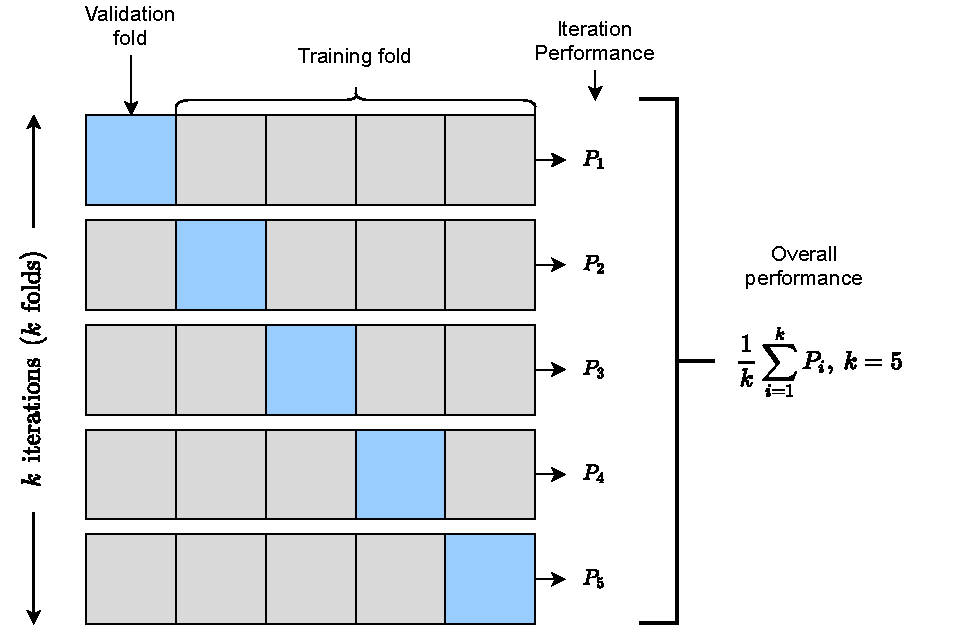
\includegraphics{Images/Background/kfold.pdf}
}    \caption[$k$-fold cross validation diagram]{$k$-fold cross validation diagram for $k=5$ folds.}
    \label{fig:kfold}
\end{figure}

Moreover, a common practice to ensure a robust model is to use \textit{$k$-fold cross validation}. This is to subdivide the training set into $k$ subsamples where one is for validation and the rest $k-1$ subsamples are for actual training. Then, the model is run over all the splits every time taking a different one for validation to finally take an average of each run. These averages can then be used to compare other models in a statistically validated way. In figure \ref{fig:kfold} a diagram of the $k$-fold cross validation process is shown.

Finally, an additional measure to prevent overfitting is the use of early stopping. Since the model has to run a number of epochs to be determined, it is possible that up to a certain number of epochs the model stops improving. Notice that a halt in improvement does not necessarily mean that the training loss does not improve, rather, it could be the case that the training set is performing better at each epoch but the validation gets worse which is a clear sign of overfitting. Hence, early stopping consists of setting a maximum number of epochs $M$ as well as a patience parameter $P$, which is the number of consecutive epochs that the model will check for improvement, stopping the process if validation loss does not improve in $P$ consecutive epochs. 

\section{Convolutional Neural Networks}

Convolutional Neural Networks (CNN) are a type of ANN that has been used widely when dealing with grid-like data. These kinds of networks work just as a regular ANN in the sense that they receive an input, perform a matrix operation with learnable weights and biases and then apply a non-linear activation. The difference lies in that CNN make use of the spatial relationships of the input which would be lost if the input were flattened to use a fully connected layer.

In figure \ref{fig:cnn} a typical CNN architecture is shown. Three distinctive parts can be identified: 

\begin{figure}
	\centering
	\begin{tikzpicture}
		\node at (0.5,-1){\begin{tabular}{c}Input\end{tabular}};
		
		\draw (0,0) -- (1,0) -- (1,1) -- (0,1) -- (0,0);
		
		\node at (3,3.5){\begin{tabular}{c}Convolutional\\ layer $1$\end{tabular}};
		
		\draw[fill=black,opacity=0.2,draw=black] (2.75,1.25) -- (3.75,1.25) -- (3.75,2.25) -- (2.75,2.25) -- (2.75,1.25);
		\draw[fill=black,opacity=0.2,draw=black] (2.5,1) -- (3.5,1) -- (3.5,2) -- (2.5,2) -- (2.5,1);
		\draw[fill=black,opacity=0.2,draw=black] (2.25,0.75) -- (3.25,0.75) -- (3.25,1.75) -- (2.25,1.75) -- (2.25,0.75);
		\draw[fill=black,opacity=0.2,draw=black] (2,0.5) -- (3,0.5) -- (3,1.5) -- (2,1.5) -- (2,0.5);
		\draw[fill=black,opacity=0.2,draw=black] (1.75,0.25) -- (2.75,0.25) -- (2.75,1.25) -- (1.75,1.25) -- (1.75,0.25);
		\draw[fill=black,opacity=0.2,draw=black] (1.5,0) -- (2.5,0) -- (2.5,1) -- (1.5,1) -- (1.5,0);
		
		\node at (4.2,-1){\begin{tabular}{c}Pooling\\layer $1$\end{tabular}};
		
		\draw[fill=black,opacity=0.2,draw=black] (5,1.25) -- (5.75,1.25) -- (5.75,2) -- (5,2) -- (5,1.25);
		\draw[fill=black,opacity=0.2,draw=black] (4.75,1) -- (5.5,1) -- (5.5,1.75) -- (4.75,1.75) -- (4.75,1);
		\draw[fill=black,opacity=0.2,draw=black] (4.5,0.75) -- (5.25,0.75) -- (5.25,1.5) -- (4.5,1.5) -- (4.5,0.75);
		\draw[fill=black,opacity=0.2,draw=black] (4.25,0.5) -- (5,0.5) -- (5,1.25) -- (4.25,1.25) -- (4.25,0.5);
		\draw[fill=black,opacity=0.2,draw=black] (4,0.25) -- (4.75,0.25) -- (4.75,1) -- (4,1) -- (4,0.25);
		\draw[fill=black,opacity=0.2,draw=black] (3.75,0) -- (4.5,0) -- (4.5,0.75) -- (3.75,0.75) -- (3.75,0);
		
		\node at (7.5,3.5){\begin{tabular}{c}Convolutional\\layer $2$\end{tabular}};
		
		\draw[fill=black,opacity=0.2,draw=black] (7.5,1.75) -- (8.25,1.75) -- (8.25,2.5) -- (7.5,2.5) -- (7.5,1.75);
		\draw[fill=black,opacity=0.2,draw=black] (7.25,1.5) -- (8,1.5) -- (8,2.25) -- (7.25,2.25) -- (7.25,1.5);
		\draw[fill=black,opacity=0.2,draw=black] (7,1.25) -- (7.75,1.25) -- (7.75,2) -- (7,2) -- (7,1.25);
		\draw[fill=black,opacity=0.2,draw=black] (6.75,1) -- (7.5,1) -- (7.5,1.75) -- (6.75,1.75) -- (6.75,1);
		\draw[fill=black,opacity=0.2,draw=black] (6.5,0.75) -- (7.25,0.75) -- (7.25,1.5) -- (6.5,1.5) -- (6.5,0.75);
		\draw[fill=black,opacity=0.2,draw=black] (6.25,0.5) -- (7,0.5) -- (7,1.25) -- (6.25,1.25) -- (6.25,0.5);
		\draw[fill=black,opacity=0.2,draw=black] (6,0.25) -- (6.75,0.25) -- (6.75,1) -- (6,1) -- (6,0.25);
		\draw[fill=black,opacity=0.2,draw=black] (5.75,0) -- (6.5,0) -- (6.5,0.75) -- (5.75,0.75) -- (5.75,0);
		
		\node at (8.5,-1){\begin{tabular}{c}Pooling\\layer $2$\end{tabular}};
		
		\draw[fill=black,opacity=0.2,draw=black] (10,1.75) -- (10.5,1.75) -- (10.5,2.25) -- (10,2.25) -- (10,1.75);
		\draw[fill=black,opacity=0.2,draw=black] (9.75,1.5) -- (10.25,1.5) -- (10.25,2) -- (9.75,2) -- (9.75,1.5);
		\draw[fill=black,opacity=0.2,draw=black] (9.5,1.25) -- (10,1.25) -- (10,1.75) -- (9.5,1.75) -- (9.5,1.25);
		\draw[fill=black,opacity=0.2,draw=black] (9.25,1) -- (9.75,1) -- (9.75,1.5) -- (9.25,1.5) -- (9.25,1);
		\draw[fill=black,opacity=0.2,draw=black] (9,0.75) -- (9.5,0.75) -- (9.5,1.25) -- (9,1.25) -- (9,0.75);
		\draw[fill=black,opacity=0.2,draw=black] (8.75,0.5) -- (9.25,0.5) -- (9.25,1) -- (8.75,1) -- (8.75,0.5);
		\draw[fill=black,opacity=0.2,draw=black] (8.5,0.25) -- (9,0.25) -- (9,0.75) -- (8.5,0.75) -- (8.5,0.25);
		\draw[fill=black,opacity=0.2,draw=black] (8.25,0) -- (8.75,0) -- (8.75,0.5) -- (8.25,0.5) -- (8.25,0);
		
		\node at (12,3.5){\begin{tabular}{c}Fully connected\\layer\end{tabular}};
		
		\draw[fill=black,draw=black,opacity=0.5] (10.5,0) -- (11,0) -- (12.5,1.75) -- (12,1.75) -- (10.5,0);
		
		\node at (13,-1){\begin{tabular}{c}Output layer\end{tabular}};
		
		\draw[fill=black,draw=black,opacity=0.5] (12.5,0.5) -- (13,0.5) -- (13.65,1.25) -- (13.15,1.25) -- (12.5,0.5);
	\end{tikzpicture}
	\caption[Architecture of a convolutional neural network]{Diagram of a CNN. The input is expected to have a grid-like structure.  The architecture consists of two convolutional blocks which include a convolutional and pooling layer. After the subsequent convolutional blocks, a fully connected layer is used to finally produce the output. Source: \url{https://davidstutz.de/illustrating-convolutional-neural-networks-in-latex-with-tikz/} \cite{conv-graphs}.}
	\label{fig:cnn}
\end{figure}

\begin{itemize}
    \item \textbf{Convolutional layer:} This layer performs a convolution operation between the input and a kernel\footnote{Also called filter.} with weights that the network can learn, these kernels have a width and height that define the window of the convolution and depth which defines the number of different outputs of the operation. The transformed data from the convolution process is called a feature map. Specifically, figure \ref{fig:filters} shows that a number of kernels is defined, as one would define the number of neurons in a fully connected layer. These kernels have a fixed size and slide through the input image or feature map and perform a convolution operation. After the convolution is done, an activation function is applied such as a ReLU, as in a regular ANN.
    
    The one dimensional convolution is defined as
    \begin{align*}
        s(t) = (x *w)(t)=\int x(\tau)w(t-\tau)d\tau
    \end{align*}
    In the context of CNN, $s(t)$ is the resulting feature map, the input is $x$ and the kernel is $w$. In practice, the input is a multidimensional array of data points, so a discrete convolution is used
    \begin{align*}
        s(t) = (x *w)(t)=\sum_{a=-\infty}^\infty x(a)w(t-a)
    \end{align*}
    It is assumed that these functions are zero in all their domain except for the actual values of the data, so the infinite sum can be computed. Furthermore, it is common to process image-like data and kernels, so a 2D version is defined as
    \begin{align*}
        S(i,j)=(I * K)(i,j)=\sum_{m}\sum_{n} I(i+m,j+n)K(m,n)
    \end{align*}
    This is called \textit{cross-correlation} and is equivalent to the convolution operation except that it is non-commutative, $S(i,j) = (I*K)(i,j)\neq (K*I) (i,j) $, but this is not an issue when implementing the network as long as the application is consistent. Figure \ref{fig:2dconv-ex} shows how this works in practice for a $2D$ input and a $3\times 3$ kernel.\\
    
    \begin{figure}
        
        \centering
        \begin{tikzpicture}

	\matrix (mtr) [matrix of nodes,row sep=-\pgflinewidth, nodes={draw}]
	{
		0 & 1 & 1 & |[fill=red!30]| 1 & |[fill=red!30]| 0 & |[fill=red!30]| 0 & 0\\
		0 & 0 & 1 & |[fill=red!30]| 1 & |[fill=red!30]| 1 & |[fill=red!30]| 0 & 0\\
		0 & 0 & 0 & |[fill=red!30]| 1 & |[fill=red!30]| 1 & |[fill=red!30]| 1 & 0\\
		0 & 0 & 0 & 1 & 1 & 0 & 0\\
		0 & 0 & 1 & 1 & 0 & 0 & 0\\
		0 & 1 & 1 & 0 & 0 & 0 & 0\\
		1 & 1 & 0 & 0 & 0 & 0 & 0\\
	};

	\draw[very thick, red] (mtr-1-4.north west) rectangle (mtr-3-6.south east);

	\node [below= of mtr-5-4.south] (lm) {$\bf I$};

	\node[right = 0.2em of mtr] (str) {$*$};

	\matrix (K) [right=0.2em of str,matrix of nodes,row sep=-\pgflinewidth, nodes={draw, fill=blue!30}]
	{
		1 & 0 & 1 \\
		0 & 1 & 0 \\
		1 & 0 & 1 \\
	};
	\node [below = of K-3-2.south] (lk) {$\bf K$};

	\node [right = 0.2em of K] (eq) {$=$};

	\matrix (ret) [right=0.2em of eq,matrix of nodes,row sep=-\pgflinewidth, nodes={draw}]
	{
		1 & 4 & 3 & |[fill=green!30]| 4 & 1\\
		1 & 2 & 4 & 3 & 3\\
		1 & 2 & 3 & 4 & 1\\
		1 & 3 & 3 & 1 & 1\\
		3 & 3 & 1 & 1 & 0\\
	};
	\node [below = of ret-4-3.south] (lim) {${\bf I} * {\bf K}$};

	\draw[very thick, green] (ret-1-4.north west) rectangle (ret-1-4.south east);

	\draw[densely dotted, blue, thick] (mtr-1-4.north west) -- (K-1-1.north west);
	\draw[densely dotted, blue, thick] (mtr-3-4.south west) -- (K-3-1.south west);
	\draw[densely dotted, blue, thick] (mtr-1-6.north east) -- (K-1-3.north east);
	\draw[densely dotted, blue, thick] (mtr-3-6.south east) -- (K-3-3.south east);

	\draw[densely dotted, green, thick] (ret-1-4.north west) -- (K-1-1.north west);
	\draw[densely dotted, green, thick] (ret-1-4.south west) -- (K-3-1.south west);
	\draw[densely dotted, green, thick] (ret-1-4.north east) -- (K-1-3.north east);
	\draw[densely dotted, green, thick] (ret-1-4.south east) -- (K-3-3.south east);

	\matrix (K) [right=0.2em of str,matrix of nodes,row sep=-\pgflinewidth, nodes={draw, fill=blue!10}]
	{
		1 & 0 & 1 \\
		0 & 1 & 0 \\
		1 & 0 & 1 \\
	};

	\draw[very thick, blue] (K-1-1.north west) rectangle (K-3-3.south east);

	\node[anchor=south east, inner sep=0.01em, blue] at (mtr-1-4.south east) (xx) {\scalebox{.5}{$\times 1$}};
	\node[anchor=south east, inner sep=0.01em, blue] at (mtr-1-5.south east) (xx) {\scalebox{.5}{$\times 0$}};
	\node[anchor=south east, inner sep=0.01em, blue] at (mtr-1-6.south east) (xx) {\scalebox{.5}{$\times 1$}};
	\node[anchor=south east, inner sep=0.01em, blue] at (mtr-2-4.south east) (xx) {\scalebox{.5}{$\times 0$}};
	\node[anchor=south east, inner sep=0.01em, blue] at (mtr-2-5.south east) (xx) {\scalebox{.5}{$\times 1$}};
	\node[anchor=south east, inner sep=0.01em, blue] at (mtr-2-6.south east) (xx) {\scalebox{.5}{$\times 0$}};
	\node[anchor=south east, inner sep=0.01em, blue] at (mtr-3-4.south east) (xx) {\scalebox{.5}{$\times 1$}};
	\node[anchor=south east, inner sep=0.01em, blue] at (mtr-3-5.south east) (xx) {\scalebox{.5}{$\times 0$}};
	\node[anchor=south east, inner sep=0.01em, blue] at (mtr-3-6.south east) (xx) {\scalebox{.5}{$\times 1$}};

\end{tikzpicture}
        \caption[Two dimensional discrete convolution example]{Two dimensional discrete convolution example where $I$ is the input, $K$ the kernel and $I*K$ is the convolution that yields the resulting feature map. Source: \url{https://github.com/PetarV-/TikZ}.}
        \label{fig:2dconv-ex}
    \end{figure}
    \begin{figure}
    	\centering
    	\begin{tikzpicture}
		\node at (1.5,4){\begin{tabular}{c}input image\\or feature map\end{tabular}};
	
		\draw (0,0) -- (3,0) -- (3,3) -- (0,3) -- (0,0);
		
		\draw (2,2) -- (2.5,2) -- (2.5,2.5) -- (2,2.5) -- (2,2);
		\draw (2,0.5) -- (2.5,0.5) -- (2.5,1) -- (2,1) -- (2,0.5);
		\draw (1,1) -- (1.5,1) -- (1.5,1.5) -- (1,1.5) -- (1,1);
		
		\draw (2.5,2) -- (7,3.25);
		\draw (2.5,2.5) -- (7,3.25);
 
		\draw (2.5,1) -- (5.75,0.25);
		\draw (2.5,0.5) -- (5.75,0.25);
		
		\draw (1.5,1.5) -- (5.5,1.25);
		\draw (1.5,1) -- (5.5,1.25);
		
		\node at (5.75,4){\begin{tabular}{c}output feature maps\end{tabular}};
		
		\draw[fill=black,opacity=0.2,draw=black] (5.5,1.5) -- (7.5,1.5) -- (7.5,3.5) -- (5.5,3.5) -- (5.5,1.5);
		\draw[fill=black,opacity=0.2,draw=black] (5,1) -- (7,1) -- (7,3) -- (5,3) -- (5,1);
		\draw[fill=black,opacity=0.2,draw=black] (4.5,0.5) -- (6.5,0.5) -- (6.5,2.5) -- (4.5,2.5) -- (4.5,0.5);
		\draw[fill=black,opacity=0.2,draw=black] (4,0) -- (6,0) -- (6,2) -- (4,2) -- (4,0);
	\end{tikzpicture}
    	\caption[Illustration of a convolutional layer]{Illustration of a convolutional layer. A number of filters with learnable parameters are applied to the input or previous feature map by using the filters as a sliding window and computing the dot product at each step. Source: \url{https://davidstutz.de/illustrating-convolutional-neural-networks-in-latex-with-tikz/} \cite{conv-graphs}.}
    	\label{fig:filters}
    \end{figure}

    In practice, it is necessary to define some parameters to apply a convolutional layer, namely the kernel size, strides and padding. The strides are the amount of pixels the kernel moves at each step while the padding defines the behavior in the borders, when part of the kernel lies outside of the input. In figures \ref{fig:no_padding_no_strides} and \ref{fig:arbitrary_padding_no_strides} examples with specific input, kernel, strides and padding are shown. Notice that all of these parameters will affect the shape of the output. 
    
    \begin{figure}
    \centering
    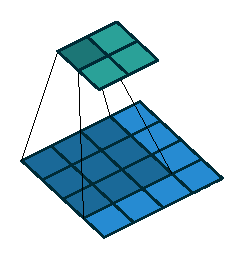
\includegraphics[width=0.24\textwidth]{Images/Background/Convolution/no_padding_no_strides_00.pdf}
    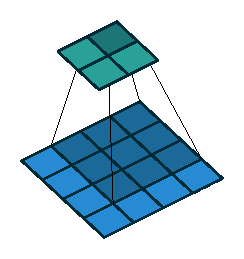
\includegraphics[width=0.24\textwidth]{Images/Background/Convolution/no_padding_no_strides_01.pdf}
    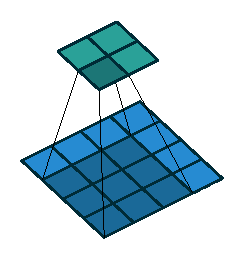
\includegraphics[width=0.24\textwidth]{Images/Background/Convolution/no_padding_no_strides_02.pdf}
    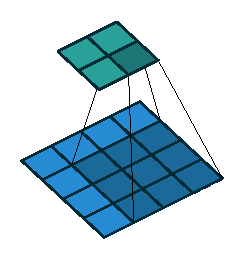
\includegraphics[width=0.24\textwidth]{Images/Background/Convolution/no_padding_no_strides_03.pdf}
    \caption[Unit strides and no padding convolution]{Convolving a $3 \times 3$ kernel over a $4 \times 4$ input using unit strides and no padding. Source: \url{https://github.com/vdumoulin/conv_arithmetic} \cite{trans-conv}.}
    \label{fig:no_padding_no_strides}
    \end{figure}
    
    \begin{figure}
        \centering
        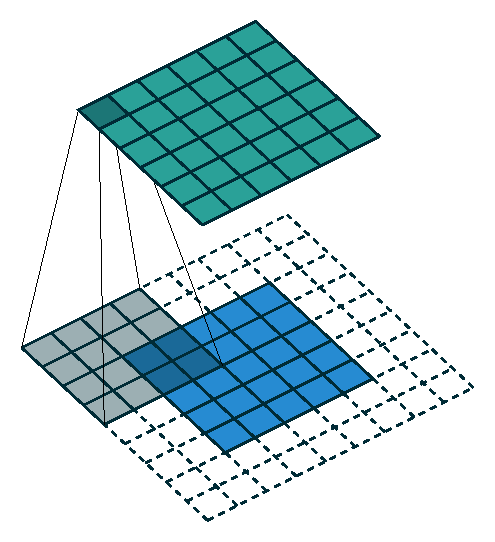
\includegraphics[width=0.24\textwidth]{Images/Background/Convolution/arbitrary_padding_no_strides_00.pdf}
        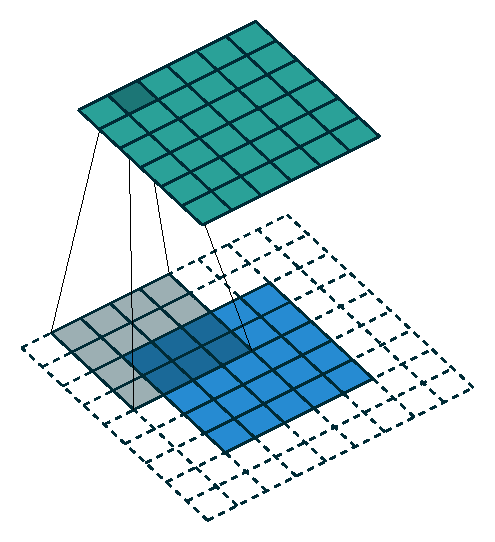
\includegraphics[width=0.24\textwidth]{Images/Background/Convolution/arbitrary_padding_no_strides_01.pdf}
        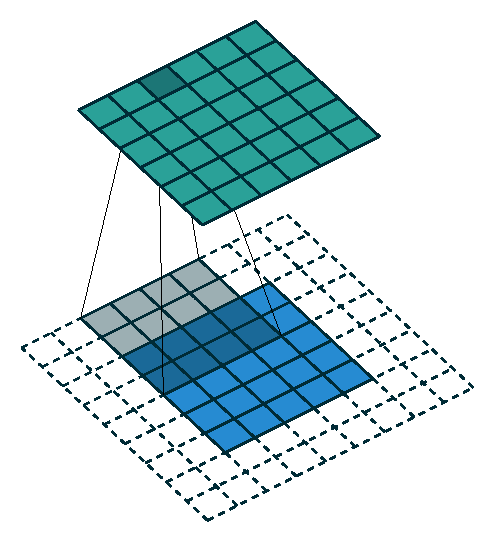
\includegraphics[width=0.24\textwidth]{Images/Background/Convolution/arbitrary_padding_no_strides_02.pdf}
        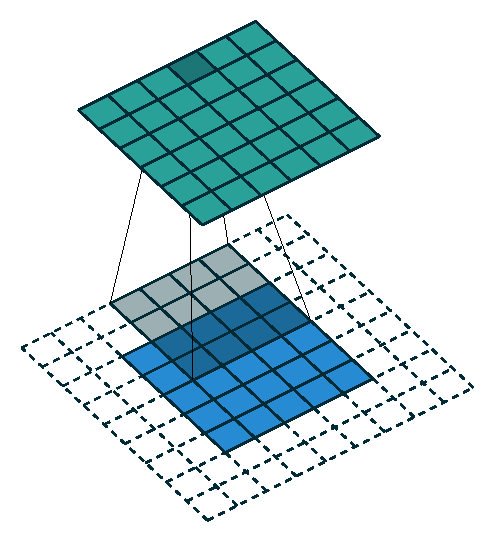
\includegraphics[width=0.24\textwidth]{Images/Background/Convolution/arbitrary_padding_no_strides_03.pdf}
        \caption[Unit strides and zero padding convolution]{Convolving a $4 \times 4$ kernel over a $5 \times 5$ input padded with a $2 \times 2$ border of zeros using unit strides. Source: \url{https://github.com/vdumoulin/conv_arithmetic} \cite{trans-conv}.}
        \label{fig:arbitrary_padding_no_strides}
    \end{figure}

    Furthermore, it is useful to define the input size ($i_j$), kernel size ($k_j$), stride size ($s_j$) and padding size ($p_j$) where each parameter is considered along axis $j$\footnote{In the case of square input, strides and padding this distinction is not necessary.}. Then, a general expression \cite{trans-conv} for the output shape is
    \begin{align*}
        o_j &= \left\lfloor \frac{i_j+2p_j-k_j}{s_j}, \right\rfloor+1 \quad \forall i,k,s,p \in \N
    \end{align*}

    \item \textbf{Pooling layer:} The pooling layer downsamples the previously convolved input, i.e. feature maps, thus reducing the dimension of the data. A commonly used type of pooling layer is the max pooling, in which a window slides through the data and takes the maximum value within the window. The way it works is very similar to a convolution in the sense that a kernel size is defined, and this kernel scans the input and applies a transformation at each step. The difference is that the transformation is not a convolution, but a downsample through the use of some statistical feature within the window (average, maximum, etc). A diagram of a pooling layer is shown in \ref{fig:maxpool}. Similar to the convolution, the kernel size and strides affect the size of the downsampled output. An expression for the output size is\footnote{Axis subindex is omitted for simplicity.} 
    \begin{align*}
        o &= \left\lfloor \frac{i-k}{s}+1, \right\rfloor+1 \quad \forall i,k,s \in \N
    \end{align*}
    \begin{figure}
	\centering
	\begin{tikzpicture}
		\node at (1.75,4.5){\begin{tabular}{c}feature maps\\layer $(l-1)$\end{tabular}};
		
		\draw[fill=black,opacity=0.2,draw=black] (1.5,1.5) -- (3.5,1.5) -- (3.5,3.5) -- (1.5,3.5) -- (1.5,1.5);
		\draw[fill=black,opacity=0.2,draw=black] (1,1) -- (3,1) -- (3,3) -- (1,3) -- (1,1);
		\draw[fill=black,opacity=0.2,draw=black] (0.5,0.5) -- (2.5,0.5) -- (2.5,2.5) -- (0.5,2.5) -- (0.5,0.5);
		\draw[fill=black,opacity=0.2,draw=black] (0,0) -- (2,0) -- (2,2) -- (0,2) -- (0,0);
		
		\draw (3.1,3.1) -- (3.4,3.1) -- (3.4,3.4) -- (3.1,3.4) -- (3.1,3.1);
		\draw (2.6,1.1) -- (2.9,1.1) -- (2.9,1.4) -- (2.6,1.4) -- (2.6,1.1);
		\draw (1.1,0.1) -- (1.4,0.1) -- (1.4,0.4) -- (1.1,0.4) -- (1.1,0.1);
		
		\draw (3.4,3.4) -- (7.8,2.8);
		\draw (3.4,3.1) -- (7.8,2.8);
		
		\draw (2.9,1.4) -- (7.3,1.2);
		\draw (2.9,1.1) -- (7.3,1.2);
		
		\draw (1.4,0.4) -- (5.9,0.3);
		\draw (1.4,0.1) -- (5.9,0.3);
		
		\node at (6.5,4.5){\begin{tabular}{c}feature maps\\layer $l$\end{tabular}};
		
		\draw[fill=black,opacity=0.2,draw=black] (6.5,1.5) -- (8,1.5) -- (8,3) -- (6.5,3) -- (6.5,1.5);
		\draw[fill=black,opacity=0.2,draw=black] (6,1) -- (7.5,1) -- (7.5,2.5) -- (6,2.5) -- (6,1);
		\draw[fill=black,opacity=0.2,draw=black] (5.5,0.5) -- (7,0.5) -- (7,2) -- (5.5,2) -- (5.5,0.5);
		\draw[fill=black,opacity=0.2,draw=black] (5,0) -- (6.5,0) -- (6.5,1.5) -- (5,1.5) -- (5,0);
	\end{tikzpicture}
	\caption[Illustration of a pooling layer]{Illustration of a pooling layer. Layer $l$ summarizes the information in layer $l-1$ through some statistical feature (maximum, average, etc). This is accomplished by defining a fixed size window and then scanning the previous layer, applying the pooling operation at each step. The number of feature maps remains the same. Source: \url{https://davidstutz.de/illustrating-convolutional-neural-networks-in-latex-with-tikz/} \cite{conv-graphs}.}
	\label{fig:maxpool}
    \end{figure}
    
    \item \textbf{Fully connected layer:} A feed forward network is used to produce the final output. Since the convolutional and pooling layers already have done the work of extracting relevant spatial features, the fully connected layers can then receive the transformed data.
\end{itemize} 

Furthermore, CNN have properties that benefit their application \cite{cnn-survey}:
\begin{itemize}
    \item \textbf{Sparse interactions:} The number of parameters is reduced compared to fully connected layers since kernels are usually much smaller than the input and this is more efficient in terms of memory usage.
    \item \textbf{Shared weights:} Weights are used multiple times in the model because kernels slide through the input while dense layers have each weight associated with only one feature.
    \item \textbf{Equivariance to translation:} The representation of the input's features is equivariant to the location of features, that is, if the input is translated, the feature maps in each layer will be translated in the same way \cite{dl-book}.
\end{itemize}

\section{Segmentation models}
An important problem in computer vision is the analysis of images or videos for segmentation and it has been addressed using different techniques, including deep learning models which are discussed in this section.

First, the segmentation task encompasses several different but related problems. The most common are: 
\begin{itemize}
    \item \textbf{Object localization:} An image with different subjects is processed and the model is expected to localize them, this is usually done using bounding boxes around every subject.
    
    \item \textbf{Semantic segmentation:} In this case, each pixel of the image is labeled as a subject, so the specific geometry is recognized as opposed to the bounding box localization.
    
    \item \textbf{Instance segmentation:} This expands the semantic segmentation by assigning labels to each instance of a subject within an image. This allows to separate subjects that would have the same label in semantic segmentation.
\end{itemize}

In figure \ref{fig:segment-types} the different types of segmentation are depicted. This thesis is concerned with the application of supervised semantic segmentation models, so the models studied aim to solve that task.

\begin{figure}
  \begin{subfigure}[b]{0.45\textwidth}
    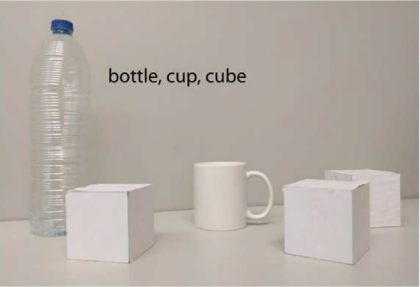
\includegraphics[width=\linewidth]{Images/Background/s1.png}
    \caption{Input image}
    \label{fig:input_img}
  \end{subfigure}
\hfill
  \begin{subfigure}[b]{0.45\textwidth}
    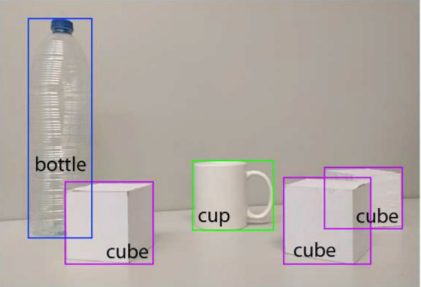
\includegraphics[width=\linewidth]{Images/Background/s2.png}
    \caption{Localization}
    \label{fig:localization}
  \end{subfigure}
  \begin{subfigure}[b]{0.45\textwidth}
    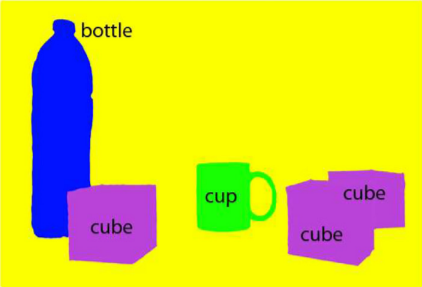
\includegraphics[width=\linewidth]{Images/Background/s3.png}
    \caption{Semantic segmentation}
    \label{fig:semantic}
  \end{subfigure}
\hfill
  \begin{subfigure}[b]{0.45\textwidth}
    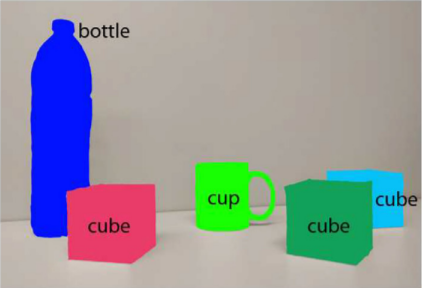
\includegraphics[width=\linewidth]{Images/Background/s4.png}
    \caption{Instance segmentation}
    \label{fig:instance}
  \end{subfigure}
  \caption[Typical segmentation tasks]{Typical segmentation tasks. Source: \textit{A survey on deep learning techniques for image and video semantic segmentation} \cite{segmentation-survey-2}.}
  \label{fig:segment-types}
\end{figure}

\subsection{Fully convolutional networks}

Fully Convolutional Networks (FCN) are ANN that only make use of convolutional and pooling layers. This type of architecture is suitable for semantic segmentation because it is possible to have a grid-like output, as opposed to a single value or array of values when fully connected layers are used in the output layer. As stated before, in semantic segmentation it is necessary to assign a label to each pixel in an image to generate groups of pixels that have some semantic or spatial relationship.

A generic FCN architecture is shown in figure \ref{fig:fcn}. The structure is composed of a contracting convolutional path in which subsequent convolutional and pooling layers are applied so the number of feature maps increases (depth) and the size of the input decreases (width and height). Then there is an expanding path in which transposed convolutions\footnote{The term “deconvolution” is sometimes used, but this is discouraged because a deconvolution is defined as the inverse of a convolution, which is different from a transposed convolution \cite{trans-conv}.} are applied and followed by regular convolutions that reduce the number of feature maps. The purpose of transposed convolutions is to upsample the feature maps so the original input shape is recovered. The output is the segmentation map which is an image of the same shape as the input and each pixel has a specific label. In a supervised approach, these labels come from whatever labels have been assigned to the training examples. 

\begin{figure}
	\centering
	\noindent\resizebox{\textwidth}{!}{
	\begin{tikzpicture}
		%\draw[use as bounding box, transparent] (-1.8,-1.8) rectangle (17.2, 3.2);

		\newcommand{\networkLayer}[9]{
			% Define the macro.
			% 1st argument: Height and width of the layer rectangle slice.
			% 2nd argument: Depth of the layer slice
			% 3rd argument: X Offset --> use it to offset layers from previously drawn layers.
			% 4th argument: Y Offset --> Use it when an output needs to be fed to multiple layers that are on the same X offset.
			% 5th argument: Z Offset --> Use to offset layers from previous 
			% 6th argument: Options for filldraw.
			% 7th argument: Text to be placed below this layer.
			% 8th argument: Name of coordinates. When name = "start" this resets the offset counter
			% 9th argument: list of nodes to connect to (previous layers)
			\xdef\totalOffset{\totalOffset}
 			\ifthenelse{\equal{#8} {start}}
 			{\FPset{totalOffset}{0}}
 			{}
 			\FPeval\currentOffset{0+(totalOffset)+(#3)}

			\def\hw{#1} % Used to distinguish input resolution for current layer.
			\def\b{0.02}
			\def\c{#2} % Width of the cube to distinguish number of input channels for current layer.
			\def\x{\currentOffset} % X offset for current layer.
			\def\y{#4} % Y offset for current layer.
			\def\z{#5} % Z offset for current layer.
			\def\inText{#7}

            % Define references to points on the cube surfaces
            \coordinate (#8_front) at  (\x+\c  , \z      , \y);
            \coordinate (#8_back) at   (\x     , \z      , \y);
            \coordinate (#8_top) at    (\x+\c/2, \z+\hw/2, \y);
            \coordinate (#8_bottom) at (\x+\c/2, \z-\hw/2, \y);
            
 			% Define cube coords
			\coordinate (blr) at (\c+\x,  -\hw/2+\z,  -\hw/2+\y); %back lower right
			\coordinate (bur) at (\c+\x,   \hw/2+\z,  -\hw/2+\y); %back upper right
			\coordinate (bul) at (0 +\x,   \hw/2+\z,  -\hw/2+\y); %back upper left
			\coordinate (fll) at (0 +\x,  -\hw/2+\z,   \hw/2+\y); %front lower left
			\coordinate (flr) at (\c+\x,  -\hw/2+\z,   \hw/2+\y); %front lower right
			\coordinate (fur) at (\c+\x,   \hw/2+\z,   \hw/2+\y); %front upper right
			\coordinate (ful) at (0 +\x,   \hw/2+\z,   \hw/2+\y); %front upper left

            % Draw connections from other points to the back of this node
            \ifthenelse{\equal{#9} {}}
 			{}{
 			    \foreach \val in #9
 			        \draw[line width=0.3mm] (\val)--(#8_back);
 			}
 			
			% Draw the layer body.
			% back plane
			\draw[line width=0.3mm](blr) -- (bur) -- (bul);
			% front plane
			\draw[line width=0.3mm](fll) -- (flr) node[midway,below, text width=2cm] {\inText} -- (fur) -- (ful) -- (fll);
			\draw[line width=0.3mm](blr) -- (flr);
			\draw[line width=0.3mm](bur) -- (fur);
			\draw[line width=0.3mm](bul) -- (ful);

			% Recolor visible surfaces
			% front plane
			\filldraw[#6] ($(fll)+(\b,\b,0)$) -- ($(flr)+(-\b,\b,0)$) -- ($(fur)+(-\b,-\b,0)$) -- ($(ful)+(\b,-\b,0)$) -- ($(fll)+(\b,\b,0)$);
			\filldraw[#6] ($(ful)+(\b,0,-\b)$) -- ($(fur)+(-\b,0,-\b)$) -- ($(bur)+(-\b,0,\b)$) -- ($(bul)+(\b,0,\b)$);

			% Colored slice.
			\ifthenelse {\equal{#6} {}}{} % Do not draw colored slice if #4 is blank.
			% Else, draw a colored slice.
			{\filldraw[#6] ($(flr)+(0,\b,-\b)$) -- ($(blr)+(0,\b,\b)$) -- ($(bur)+(0,-\b,\b)$) -- ($(fur)+(0,-\b,-\b)$);}

			\FPeval\totalOffset{0+(currentOffset)+\c}
		}
		
	%\networkLayer{2.0}{0.5}{0.0}{0.0}{2.5}{color=red!50}{}{start}{}
	%\networkLayer{2.0}{0.25}{1.5}{0.0}{0.0}{color=green!50}{}{bot}{{start_front}}
	%\networkLayer{2.0}{0.25}{0.15}{0.0}{0.0}{color=green!50}{}{}{}
	%\networkLayer{2.0}{0.5}{0.15}{0.0}{0.0}{color=green!50}{}{end}{}
	%\networkLayer{2.0}{0.5}{-(2.8)/2}{0.0}{5.0}{color=green!50}{}{top}{{start_front}}
	%\networkLayer{2.0}{0.5}{2.0}{0.0}{2.5}{color=blue!50}{}{add}{{end_front,top_front}}
	%\networkLayer{1.0}{0.5}{0.15}{0.0}{2.5}{color=blue!50}{}{}{}
	%\networkLayer{0.75}{0.5}{0.15}{0.0}{2.5}{color=blue!50}{}{}{}
	%\networkLayer{0.5}{0.5}{0.15}{0.0}{2.5}{color=blue!50}{}{}{}
			% INPUT
		\networkLayer{3.0}{0.03}{0.0}{0.0}{0.0}{color=gray!80}{Input}{start}{}

		% ENCODER
		\networkLayer{3.0}{0.1}{0.5}{0.0}{0.0}{color=white}{}{}{}    % S1
		\networkLayer{2.5}{0.1}{0.1}{0.0}{0.0}{color=white}{}{}{}        % S2
		\networkLayer{2.5}{0.2}{0.1}{0.0}{0.0}{color=white}{}{}{}    % S1
		\networkLayer{2.0}{0.2}{0.1}{0.0}{0.0}{color=white}{}{}{}        % S2
		\networkLayer{2.0}{0.4}{0.1}{0.0}{0.0}{color=white}{}{}{}    % S1
		\networkLayer{1.5}{0.4}{0.1}{0.0}{0.0}{color=white}{}{}{}        % S2
		\networkLayer{1.5}{0.8}{0.1}{0.0}{0.0}{color=white}{}{}{}    % S1
		\networkLayer{1.0}{0.8}{0.1}{0.0}{0.0}{color=white}{\hspace{15pt}pool}{}{}        % S2
		\networkLayer{1.0}{1.5}{0.1}{0.0}{0.0}{color=white}{\hspace{15pt}conv}{}{}    % S1
		\networkLayer{0.7}{1.5}{0.1}{0.0}{0.0}{color=white}{}{mid}{}        % S2


		\networkLayer{0.7}{2}{0.1}{0.0}{0.0}{color=blue!50}{}{}{}

		% DECODER
		\networkLayer{1.0}{2}{0.1}{0.0}{0.0}{color=white}{\hspace{-5pt}transposed conv}{}{} % S1
		\networkLayer{1.0}{1.5}{0.1}{0.0}{0.0}{color=white}{}{}{}       % S2
		\networkLayer{1.5}{1.5}{0.1}{0.0}{0.0}{color=white}{}{}{} % S1
		\networkLayer{1.5}{0.8}{0.1}{0.0}{0.0}{color=white}{conv}{}{}       % S2
		\networkLayer{2.0}{0.8}{0.1}{0.0}{0.0}{color=white}{}{}{}       % S1
		\networkLayer{2.0}{0.4}{0.1}{0.0}{0.0}{color=white}{}{}{}       % S2
		\networkLayer{2.5}{0.4}{0.1}{0.0}{0.0}{color=white}{}{}{}       % S1
		\networkLayer{2.5}{0.2}{0.1}{0.0}{0.0}{color=white}{}{}{}       % S2
		\networkLayer{3.0}{0.2}{0.1}{0.0}{0.0}{color=white}{}{}{}       % S1
		\networkLayer{3.0}{0.1}{0.1}{0.0}{0.0}{color=white}{}{}{}       % S2

		% OUTPUT
		\networkLayer{3.0}{0.05}{0.9}{0.0}{0.0}{color=red!40}{Output}{}{}          % Pixelwise segmentation with classes.

	\end{tikzpicture}
	}
	\caption[Illustration of a fully convolutional network]{Illustration of a FCN. First, subsequent convolution and pooling layers are applied. In the convolutions the feature maps are added (more length in the figure) while maintaining height and width, then the pooling layer reduces the size while keeping the same number of feature maps. In the expanding path, a transposed convolution is applied which upsamples the feature maps, then a normal convolution is applied reducing the number of feature maps. Source: Adapted from \url{https://github.com/jettan/tikz_cnn}.}
	\label{fig:fcn}
\end{figure}

The main feature of a FCN is the upsampling layer in which the transposed convolution is applied, because without such an operation, it would no be possible to recover the shape of the input. This could be solved by not using pooling layers and maintaining the shape throughout the network, but this would be computationally expensive because the number of parameters would be really large, and one of the benefits of CNN is the possibility to reduce the number of parameters by using small filters compared to the input size.

\subsection{Transposed convolution}
The transposed convolution operation functions in the opposite way of a pooling layer, thus upsampling the input. For this, a kernel with trainable parameters is used. Note that since this is not the inverse of a convolution, the result is just a new collection of feature maps that recovers the shape of the previous layer, but does not have the same parameter values.

As an example, let us consider the convolution shown in figure \ref{fig:no_padding_no_strides}. If we write the convolution as a vector-matrix multiplication, the kernel can be written as
\setcounter{MaxMatrixCols}{20}
\begin{align*}
\resizebox{.98\hsize}{!}{$
   \mathbf{C} =\begin{pmatrix}
    w_{0,0} & w_{0,1} & w_{0,2} & 0       & w_{1,0} & w_{1,1} & w_{1,2} & 0       &
    w_{2,0} & w_{2,1} & w_{2,2} & 0       & 0       & 0       & 0       & 0       \\
    0       & w_{0,0} & w_{0,1} & w_{0,2} & 0       & w_{1,0} & w_{1,1} & w_{1,2} &
    0       & w_{2,0} & w_{2,1} & w_{2,2} & 0       & 0       & 0       & 0       \\
    0       & 0       & 0       & 0       & w_{0,0} & w_{0,1} & w_{0,2} & 0       &
    w_{1,0} & w_{1,1} & w_{1,2} & 0       & w_{2,0} & w_{2,1} & w_{2,2} & 0       \\
    0       & 0       & 0       & 0       & 0       & w_{0,0} & w_{0,1} & w_{0,2} &
    0       & w_{1,0} & w_{1,1} & w_{1,2} & 0       & w_{2,0} & w_{2,1} & w_{2,2} \\
    \end{pmatrix}$}
\end{align*}
where $w_{ij}$ is the weight of the kernel located in row $i$ and column $j$. Then, the convolution can be computed by flattening the input so that it becomes a $16-$dimensional vector. The result is going to be a $4-$dimensional vector which can be reshaped to $2\times2$ to get the matrix form. With this in mind, notice that in the forward pass, the convolution consists in multiplying by $\mathbf{C}$ while in the backward pass to propagate the error it is necessary to multiply by $\mathbf{C}^T$. Hence, the weight matrix defines both the forward and backward pass of the network.

Now consider the idea behind transposed convolution which is to take a small matrix, applying a transformation and obtaining a larger matrix maintaining the number of feature maps. This is precisely what happens when in the backward pass $\mathbf{C}^T$ is applied. Then, multiplying by $\mathbf{C}^T$ is a transposed convolution by definition if $\mathbf{C}^T$ is applied in the forward pass instead of the backward pass.

In general, the process can be thought of as having an input matrix in which every data point is multiplied by the kernel and then summed over the corresponding values. This is equivalent\footnote{This is useful as a concept, but is not used when programming because many of the operations are useless zero multiplications.} to a regular convolution over a fully padded input\footnote{This means the input is padded such that the kernel can overlap its last value (bottom-right) with the first of the input (top-left).} as shown in figure \ref{fig:no_padding_no_strides_transposed} which is a $2\times 2$ input in which a transposed convolution is applied with a $3\times 3$ kernel to produce a $4\times 4$ output or equivalently, a $6 \times 6$ (padded) input convolved with a $3\times 3$ kernel.

\begin{figure}
    \centering
    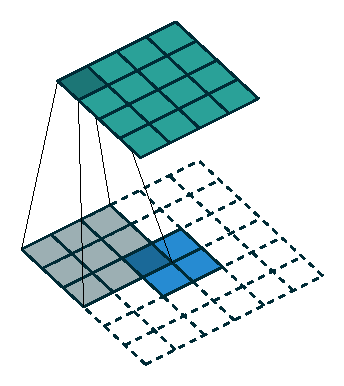
\includegraphics[width=0.24\textwidth]{Images/Background/Convolution/no_padding_no_strides_transposed_00.pdf}
    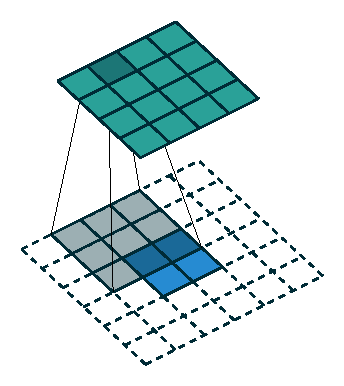
\includegraphics[width=0.24\textwidth]{Images/Background/Convolution/no_padding_no_strides_transposed_01.pdf}
    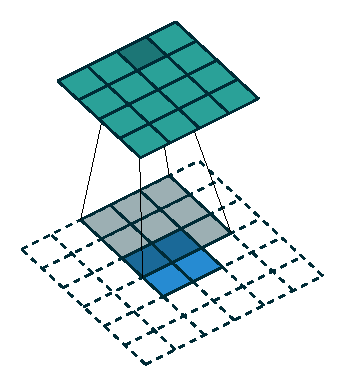
\includegraphics[width=0.24\textwidth]{Images/Background/Convolution/no_padding_no_strides_transposed_02.pdf}
    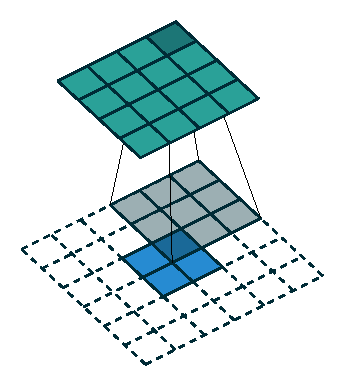
\includegraphics[width=0.24\textwidth]{Images/Background/Convolution/no_padding_no_strides_transposed_03.pdf}
    \caption[Example of a transposed convolution]{Transposed convolution of a $2\times 2$ input with a $3\times 3$ kernel to produce a $4\times 4$ output. This is equivalent to a regular convolution of a $6\times 6$ input with a $2\times 2$ padding with the same kernel. Source: \url{https://github.com/vdumoulin/conv_arithmetic} \cite{trans-conv}.}
    \label{fig:no_padding_no_strides_transposed}
\end{figure}

\subsection{Residual connections}

As of now, the networks discussed have all been connected using adjacent layers which means every node in one layer is connected with every node in the next layer, no connections are missing and no connections with other layers are added. Nonetheless, a trick that has proven to be very effective when training ANN is the use of residual connections, allowing to achieve state of the art results in a wide range of tasks. These connections consist in having a connection with deeper layers of the network, so a neuron $n$ in layer $l$ can be connected with layer $l+1$ as usual and with other layers $l+r$, $r\geq 1$.

Before residual connections were developed, some deep networks performed worse than shallow ones despite the fact that in theory neural networks are universal approximators \cite{Hornik, Cybenko}, which means that it is possible to approximate any function in a compact domain with an arbitrary small error given enough neural units. Particularly, there was a saturation in accuracy, that is the accuracy improved with depth up to a certain point at which accuracy began to decrease. This is called the degradation problem \cite{res-connection}.

Specifically when a shallow network performs better than a deep one, an intuitive approach would be to allow the deep network to skip some layers so that it can mimic the behavior of a shallow network if needed. Then, if a layer activation is small, an identity mapping can be added so that the gradient does not vanish and the network can make use of that layer's level of abstraction. In figure \ref{fig:res-connection} a residual connection is shown. 

\begin{figure}
    \centering
    \begin{tikzpicture}
    
    \node[rectangle, draw] (n1) at (0,0) {weight layer};
    \node[rectangle, draw] (n2) at (0,-1.5) {weight layer};
    \node[circle, draw, scale =.6, thick] (n3) at (0,-3) {$\mathbf{+}$};
    
    \draw[thick, ->] (0,1) -- (n1) node[midway, left] (a1) {$x$};
    \draw[thick, ->] (n1) -- (n2) node[midway, left] {$\F (x)$} node[midway, right] {$ReLU$};
    \draw[thick, ->] (n2) -- (n3);
    
    \draw[thick, ->,rounded corners] (a1) -- node[]{} (2,.7) |- (n3);

    \draw[thick, ->] (n3) -- (0,-4) node[midway, right] {$ReLU$};
    
    \draw (-1.3,-3) node[] {$F(x) + x$};
    \draw (3,-2) node[] {$x$};
    \draw[thick,->] (n1) -- (n2);
\end{tikzpicture}
    \caption[Residual connection diagram]{Residual connection diagram. Source: Adapted from \textit{Deep residual learning for image recognition} \cite{res-connection}.}
    \label{fig:res-connection}
\end{figure}

In the context of FCN, these residual connections are called \textit{skip layers}, which also skip connections to further layers in the network, but do so by concatenating layers as opposed to the sum shown in \ref{fig:res-connection}. On a semantic level, what the network does when convolving and pooling is extracting more high-level representations of the input. Then, what the skip layers do is recover the layers' low-level information which is the context needed to reconstruct when upsampling \cite{Ronneberger}.